\section{Facts}
\label{sec:facts}

A fact is the smallest unit of information in an XBRL report. 
The word "Fact" is a term used to describe an individual piece of financial of business information within an XBRL instance document. 
This section aims to represent facts and its supporting concepts in a way that is in line with the OIM.

Lets consider a simplified example involving a financial report of Microsoft Corporation for the fiscal year 2022.
Microsoft's annual report can be found on the company's website\footnote{https://www.microsoft.com/investor/reports/ar22/index.html}.
It contains a lot of information about the company's financial situation, as well as information about the company's business activities.
For this example, we will only consider the company's revenue for the fiscal year 2022.
Microsoft chose to report this information as follows:

\begin{figure}[H]
    \centering
    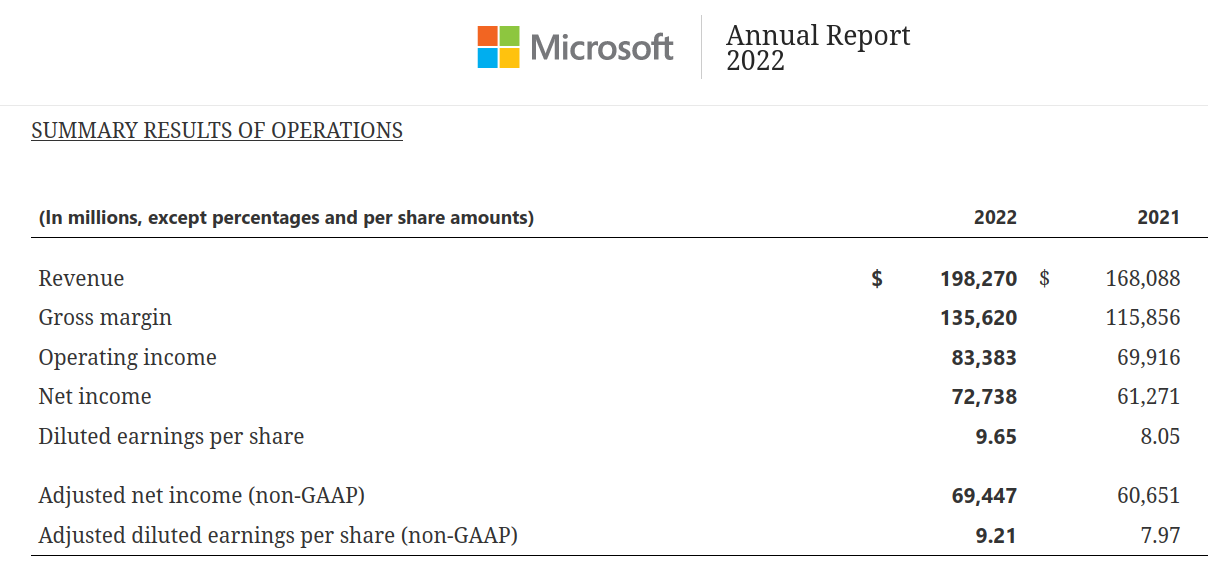
\includegraphics[width=0.75\textwidth]{images/microsoft_annual_report_2022.png}
    \caption{Microsoft's summary results of operations for the fiscal year 2021 and 2022}
    \label{fig:microsoft_annual_report_2022}
    \cite{microsoft2022ar}
\end{figure}

This table contains multiple facts about Microsoft for both fiscal years 2021 and 2022, as seen by the horizontal axis.
The vertical axis describes what is being reported. The "what is being reported" part is called the \textbf{concept} of a fact.
It reports the values for the concepts "Revenue", "Gross margin", "Operating income", \dots for both fiscal years.
In summary, the table contains 14 facts across 7 concepts for 2 fiscal years.

For now, let us focus on the top left fact, which reports the company's revenue for the fiscal year 2022.
In XBRL, a corresponding fact would be represented as follows:

\begin{itemize}
    \item \textbf{Concept:} Revenue
    \item \textbf{Entity:} Microsoft Corporation
    \item \textbf{Period:} from 2022-04-01 to 2023-03-31 \footnote{Refers to the fiscal year 2022, which starts on April 1, 2022 and ends on March 31, 2023}
    \item \textbf{Unit:} USD
    \item \textbf{Value:} 198'270'000 \footnote{https://www.microsoft.com/investor/reports/ar22/index.html}
\end{itemize}

In this example:

\begin{itemize}
    \item The \textbf{concept} refers \textit{what} is being reported. 
    In this case, "Revenue" indicates that the fact is reporting information about the company's revenue.
    \item The \textbf{entity} refers to \textit{who} is reporting. 
    In the case of our example, the entity is "Microsoft Corporation". 
    In our example this is implicit, since we are looking at Microsoft's annual report.
    However, the entity of a fact has to be explicitly stated in an XBRL report.
    \item The \textbf{period} refers to \textit{when} the information is being reported.
    The period is defined as the fiscal year 2022.
    This is indicated by the column header "2022" in the table.
    \item The \textbf{unit} refers to \textit{how} the information is being reported.
    In this example, the unit is "USD", which indicates that the information is being reported in US dollars.
    The unit is indicated by the dollar sign \$ in the table.
    \item The \textbf{value} refers to \textit{how much} is being reported.
    According to Microsoft's 2022 annual report, the company's revenue for the fiscal year 2022 was around 198 billion US dollars.
\end{itemize}

The concept, entity, period and unit of a fact are called its \textbf{aspects}. 
If necessary, additional aspects can be defined for a fact. 
These additional aspects are called \textbf{dimensions} and will be covered in section \ref{sec:hypercubes}
The aspects that are not dimensions are called \textbf{core aspects}. 
Even though the name suggests otherwise, core aspects are not all mandatory for a fact.
The only mandatory core aspect is the concept.